\documentclass[../main.tex]{subfiles}
\graphicspath{{\subfix{../Images/}}}
\begin{document}
\section{Assumed Knowledge}

\subsection{Algebra}
\subsubsection{Completing the Square}
\boxedeq{ax^{2}+bx+c = a\left(x+\frac{b}{2a}\right)^{2}+c-a\left(\frac{b}{2a}\right)^{2}}
Min/Max Point \(\displaystyle \to \left(-\frac{b}{2a}, c-a\left(\frac{b}{2a}\right)^{2}\right)\)

\subsubsection{Nature of Roots}
\begin{align*}
    Discriminant < 0 &\implies \text{No \textbf{Real} Roots}\\
    Discriminant = 0 &\implies \text{2 \textbf{Equal} Roots}\\
    Discriminant > 0 &\implies \text{2 \textbf{Distinct} Roots}
\end{align*}

\subsubsection{Vieta's Formulas (Degree of 2)}
Suppose that \(\alpha + \beta\) are the two roots of \\
\(\displaystyle ax^{2}+bx+c=0, \, a\neq0\) \\\\
Sum of roots = \(\alpha + \beta\) = \(\displaystyle -\frac{b}{a}\) \\\\
Product of roots = \(\alpha\beta\) = \(\displaystyle \frac{c}{a}\)

\subsubsection{General Vieta's formulas}


\subsubsection{Polymonials}
Expansions:
\begin{align*}
    (a \pm b)^{2} &= a^{2}\pm 2ab+b^{2} \\
    (a \pm b)^{3} &= a^{3}\pm 3a^{2}b+3ab^{2}\pm b^{3} \\
    a^{2}-b^{2} &= (a+b)(a-b) \\
    a^{3}\pm b^{3} &= (a\pm b)\left(a^{2} \mp ab+b^{2}\right) \\
\end{align*}
Binomial Formula:
\boxedeq{(a+b)^{n} = \sum_{r=0}^{n} {\binom{n}{r}a^{n-r}(b)^{r}}}

\newpage

\subsubsection{Partial Fractions}
\begin{align*}
    \displaystyle \frac{f(x)}{(ax+b)(cx+d)} &= \frac{A}{ax+b} + \frac{B}{cx+d} \, , \, A,B \in \mathbb{R} \\
    \displaystyle \frac{f(x)}{(ax+b)(cx+d)^{2}} &= \frac{A}{ax+b} + \frac{B}{cx+d} + \frac{C}{(cx+d)^{2}} \, , \, A,B,C \in \mathbb{R} \\
    \displaystyle \frac{f(x)}{(ax+b)(cx^2+d)} &= \frac{A}{ax+b} + \frac{Bx+C}{cx^{2}+d} \, , \, A,B,C \in \mathbb{R}
\end{align*}

\subsubsection{Factor \& Remainder Theorem}
Given a polynomial \(f(x)\), \\
If \(\displaystyle f\left(\frac{b}{a}\right)=0, \, a,b \in \mathbb{R}, a\neq 0\), \((ax-b)\) is \textbf{factor} of \(f(x)\) \\\\
If \(\displaystyle f\left(\frac{b}{a}\right)=c, \, a,b \in \mathbb{R}, a\neq 0\), the \textbf{remainder} of \(f(x)\) \\
divided by \((ax-b)\) is \(c\)


\subsubsection{Logarithmic \& Exponential}
\begin{tikzpicture}[scale=0.2]
    \tzaxes*(-7,-7)(15,15){\(x\)}{\(y\)}
    \def\Fx{2^\x}
    \tzfn[blue,thick]\Fx[-5:ln(12)/ln(2)]{\(f(x)=a^x\)}[ar]
    \tzfn'[red,thick]\Fx[-5:ln(12)/ln(2)]{\(f(x)=\log_{a}{x}\)}[ar]
    \tzfn[dashed]{\x}[-5:12]
\end{tikzpicture} \\

\begin{center}
    In General : \(y=a^{x} \iff x=log_{a}(y), \, a>0, \, a \neq 1\)
\end{center}

\begin{tabularx}{0.55\textwidth} {
    | >{\centering\arraybackslash}X
    | >{\centering\arraybackslash}X | }
    \hline
    \textbf{Exponential} & \textbf{Logarithmic} \\
    \hline
    \(\forall x \in \mathbb{R}, \, f(x)>0\) & \(D_{f} = \mathbb{R}^{+}\) \\
    y-intercept : \(y=1\) & x-intercept : \(x=1\) \\
    \(y=0\) is an asymptote & \(x=0\) is an asymptote \\
    \(f(x)\) is increasing for \(a>1\) & \(f(x)\) is increasing for \(a>1\) \\
    \(f(x)\) is decreasing for \(0<a<1\) & \(f(x)\) is decreasing for \(0<a<1\) \\
    \hline
\end{tabularx} \\\\

\begin{tabularx}{0.55\textwidth} {
    | >{\centering\arraybackslash}X
    | >{\centering\arraybackslash}X | }
    \hline
    \textbf{Rules of Indices} & \textbf{Laws of Logarithm} \\
    \hline
    If \(a,b,m \in \mathbb{R}^{+}\) & If \(a,m,n \in \mathbb{R}^{+}, \, a>0, \, a \neq 1\) \\
    \(a^{m}*a^{n}=a^{m+n}\) & \(\log_{a}{mn}=\log_{a}{m}+\log_{a}{n}\) \\
    \(a^{m}\div a^{n}=a^{m-n}\) & \(\log_{a}{\displaystyle \frac{m}{n}}=\log_{a}{m}-\log_{a}{n}\) \\
    \(\left(a^{m}\right)^{n}=a^{mn}\) & \(\log_{a}{m^{n}}=n\log_{a}{m}\) \\
    \(a^{m}*b^{m}=(a+b)^{m}\) & \(\log_{n}{m}=\displaystyle \frac{\log_{a}{m}}{\log_{a}{n}}\)\\
    \(a^{m}\div b^{m}=\left(\displaystyle \frac{a}{b}\right)^{m}\) & \\
    \hline
\end{tabularx} \\

\subsubsection{Modulus}
\begin{tikzpicture}[scale=0.2]
    \tzaxes*(-12,-12)(12,12){\(x\)}{\(y\)}
    \def\Fx{abs(\x)}
    \tzfn[blue,thick]\Fx[-9:9]{\(f(x)=|x|\)}[ar]
    \tzfn[dashed]{\x}[-9:0]
\end{tikzpicture} \\\\
Generally, the modulus function is defined as \\
\[|f(x)| =
    \begin{cases}
    f(x) & \text{if } x \geq 0 \\
    -f(x) & \text{if } x < 0
    \end{cases}
\]

\subsection{Trigonometry}

\subsubsection{Trigo Ratios for a General Angle}
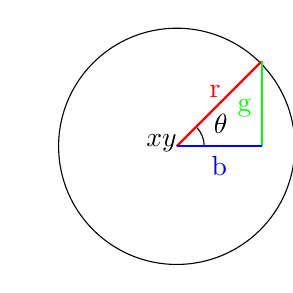
\begin{tikzpicture}[scale=1]
    \tzaxes*(-2,-2)(2,2){\(x\)}{\(y\)}
    \draw (0,0) circle [radius=1.5];
    \draw (0.35,0) arc (0:45:0.35) node[pos=0.15, above right] {\(\theta\)};
    \draw[red, thick] (0,0) -- (1.08,1.08) node[pos=0.45, above] {r};
    \draw[green, thick] (1.08,1.08) -- (1.08,0) node[pos=0.55, left] {g};
    \draw[blue, thick] (0,0) -- (1.08,0) node[pos=0.5, below] {b};
\end{tikzpicture} \\
\begin{alignat*}{2}
    \displaystyle \hspace*{10pt}\sin{\theta} &= \frac{g}{r} \hspace*{15pt} && \csc{\theta} = \frac{r}{g} \\
    \displaystyle \cos{\theta} &= \frac{b}{r} \hspace*{15pt} && \sec{\theta} = \frac{r}{b} \\
    \displaystyle \tan{\theta} &= \frac{g}{b} \hspace*{15pt} && \cot{\theta} = \frac{b}{g} \\
\end{alignat*}

\subsubsection{Principal Values}
\begin{alignat*}{2}
    \displaystyle -\frac{\pi}{2} &\leq \sin^{-1}{x} &&\leq \frac{\pi}{2} \text{ where } x \in [-1,1] \\
    \displaystyle 0 &\leq \sin^{-1}{x} &&\leq \pi \text{ where } x \in [-1,1] \\
    \displaystyle -\frac{\pi}{2} &< \tan^{-1}{x} &&< \frac{\pi}{2} \text{ where } x \in \mathbb{R} \\
\end{alignat*}

\newpage

\subsubsection{Graphs of Trigo Functions}
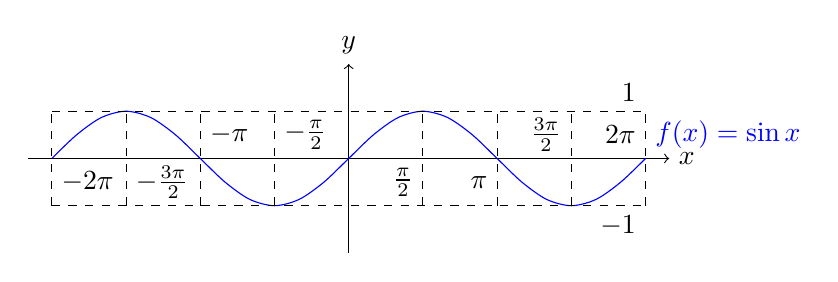
\begin{tikzpicture}[scale=0.6]
    % axes
    \draw[->] (-2*pi-0.5,0) -- (2*pi+0.5,0) node[right] {\(x\)};
    \draw[->] (0,-2) -- (0,2) node[above] {\(y\)};
    % sine curve
    \draw[domain=-2*pi:2*pi,smooth,variable=\x,blue] plot ({\x},{sin(\x r)}) node[above right] {\(f(x)=\sin{x}\)};
    % pi/2 and -pi/2
    \draw[dashed] (-pi/2,-1) -- (-pi/2,1) node[pos=0.75, right] {\(-\frac{\pi}{2}\)};
    \draw[dashed] (pi/2,-1) -- (pi/2,1) node[pos=0.25, left] {\(\frac{\pi}{2}\)};
    % pi and -pi
    \draw[dashed] (-pi,-1) -- (-pi,1) node[pos=0.75, right] {\(-\pi\)};
    \draw[dashed] (pi,-1) -- (pi,1) node[pos=0.25, left] {\(\pi\)};
    % 3pi/2 and -3pi/2
    \draw[dashed] (-3*pi/2,-1) -- (-3*pi/2,1) node[pos=0.25, right] {\(-\frac{3\pi}{2}\)};
    \draw[dashed] (3*pi/2,-1) -- (3*pi/2,1) node[pos=0.75, left] {\(\frac{3\pi}{2}\)};
    % 2pi and -2pi
    \draw[dashed] (-2*pi,-1) -- (-2*pi,1) node[pos=0.25, right] {\(-2\pi\)};
    \draw[dashed] (2*pi,-1) -- (2*pi,1) node[pos=0.75, left] {\(2\pi\)};
    % 1 and -1
    \draw[dashed] (-2*pi,1) -- (2*pi,1) node[above left] {\(1\)};
    \draw[dashed] (-2*pi,-1) -- (2*pi,-1) node[below left] {\(-1\)};
\end{tikzpicture}\\
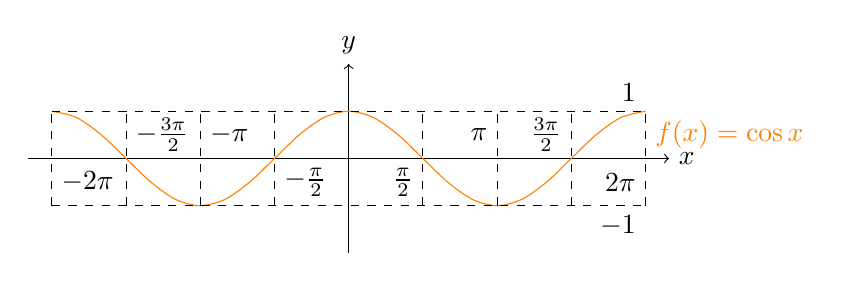
\begin{tikzpicture}[scale=0.6]
    % axes
    \draw[->] (-2*pi-0.5,0) -- (2*pi+0.5,0) node[right] {\(x\)};
    \draw[->] (0,-2) -- (0,2) node[above] {\(y\)};
    % sine curve
    \draw[domain=-2*pi:2*pi,smooth,variable=\x,orange] plot ({\x},{cos(\x r)}) node[below right] {\(f(x)=\cos{x}\)};
    % pi/2 and -pi/2
    \draw[dashed] (-pi/2,-1) -- (-pi/2,1) node[pos=0.25, right] {\(-\frac{\pi}{2}\)};
    \draw[dashed] (pi/2,-1) -- (pi/2,1) node[pos=0.25, left] {\(\frac{\pi}{2}\)};
    % pi and -pi
    \draw[dashed] (-pi,-1) -- (-pi,1) node[pos=0.75, right] {\(-\pi\)};
    \draw[dashed] (pi,-1) -- (pi,1) node[pos=0.75, left] {\(\pi\)};
    % 3pi/2 and -3pi/2
    \draw[dashed] (-3*pi/2,-1) -- (-3*pi/2,1) node[pos=0.75, right] {\(-\frac{3\pi}{2}\)};
    \draw[dashed] (3*pi/2,-1) -- (3*pi/2,1) node[pos=0.75, left] {\(\frac{3\pi}{2}\)};
    % 2pi and -2pi
    \draw[dashed] (-2*pi,-1) -- (-2*pi,1) node[pos=0.25, right] {\(-2\pi\)};
    \draw[dashed] (2*pi,-1) -- (2*pi,1) node[pos=0.25, left] {\(2\pi\)};
    % 1 and -1
    \draw[dashed] (-2*pi,1) -- (2*pi,1) node[above left] {\(1\)};
    \draw[dashed] (-2*pi,-1) -- (2*pi,-1) node[below left] {\(-1\)};
\end{tikzpicture}\\
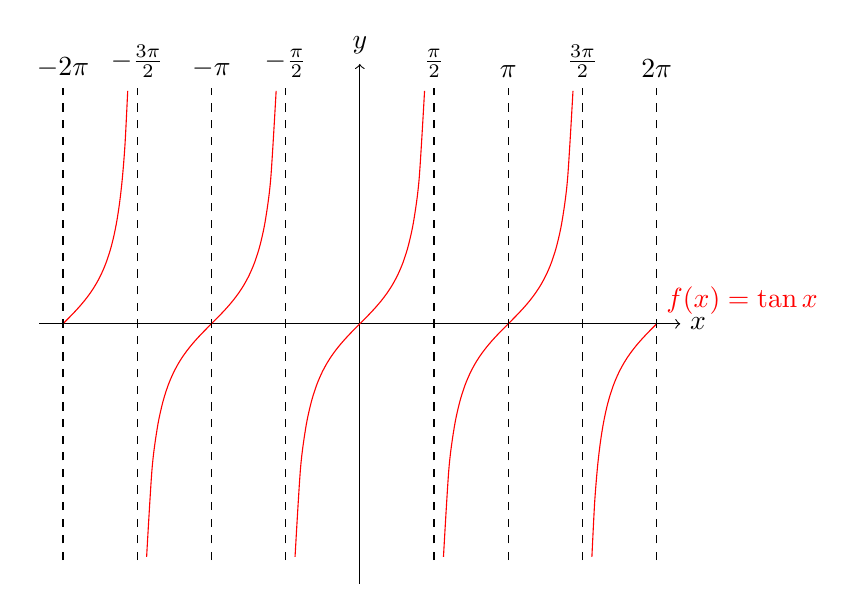
\begin{tikzpicture}[scale=0.6]
    % axes
    \draw[->] (-2*pi-0.5,0) -- (2*pi+0.5,0) node[right] {\(x\)};
    \draw[->] (0,-5.5) -- (0,5.5) node[above] {\(y\)};
    % tangent curve
    \draw[domain=-2*pi:-3*pi/2-0.2,smooth,variable=\x,red] plot ({\x},{tan(\x r)});
    \draw[domain=-3*pi/2+0.2:-pi/2-0.2,smooth,variable=\x,red] plot ({\x},{tan(\x r)});
    \draw[domain=-pi/2+0.2:pi/2-0.2,smooth,variable=\x,red] plot ({\x},{tan(\x r)});
    \draw[domain=pi/2+0.2:3*pi/2-0.2,smooth,variable=\x,red] plot ({\x},{tan(\x r)});
    \draw[domain=3*pi/2+0.2:2*pi,smooth,variable=\x,red] plot ({\x},{tan(\x r)}) node[above right] {\(f(x)=\tan{x}\)};
    % pi/2 and -pi/2
    \draw[dashed] (-pi/2,-5) -- (-pi/2,5) node[above] {\(-\frac{\pi}{2}\)};
    \draw[dashed] (pi/2,-5) -- (pi/2,5) node[above] {\(\frac{\pi}{2}\)};
    % pi and -pi
    \draw[dashed] (-pi,-5) -- (-pi,5) node[above] {\(-\pi\)};
    \draw[dashed] (pi,-5) -- (pi,5) node[above] {\(\pi\)};
    % 3pi/2 and -3pi/2
    \draw[dashed] (-3*pi/2,-5) -- (-3*pi/2,5) node[above] {\(-\frac{3\pi}{2}\)};
    \draw[dashed] (3*pi/2,-5) -- (3*pi/2,5) node[above] {\(\frac{3\pi}{2}\)};
    % 2pi and -2pi
    \draw[dashed] (-2*pi,-5) -- (-2*pi,5) node[above] {\(-2\pi\)};
    \draw[dashed] (2*pi,-5) -- (2*pi,5) node[above] {\(2\pi\)};
\end{tikzpicture}

\subsubsection{Sine \& Cosine Rules}
Given any triangle with sides of length \(a,b,c\) and \\
opposite angles \(A,B,C\)
\begin{center}
    \(\displaystyle \frac{a}{\sin{A}} = \frac{b}{\sin{B}}=\frac{c}{\sin{C}}\) \\ \vspace*{5pt}
    \(\displaystyle a^{2} = b^{2}+c^{2}-2(b)(c)\cos{A}\) \\ \vspace*{5pt}
    \(\displaystyle \cos{A} = \frac{b^{2}+c^{2}-a^{2}}{2(b)(c)}\)
\end{center}

\subsubsection{R-Formula}
A Sum or difference of Sines and cosines can be represented with a single trig function if they have the same angles
\boxedeq{a\sin{\theta} \pm b\cos{\theta} = \sin{(\theta \pm \alpha)}} \boxedeq{a\cos{\theta} \mp b\cos{\theta} = \cos{(\theta \pm \alpha)}}
\begin{equation*}
    \displaystyle R = \sqrt{a^{2}+b^{2}} \text{ \& } \alpha = \tan^{-1}{\left(\frac{b}{a}\right)}
\end{equation*}

\newpage

\subsubsection{Basic Identities}
\begin{align*}
    \displaystyle \text{Area of Triangle} &= \frac{1}{2}(a)(b)\sin{\theta} \\
    \displaystyle \sin^{2}{\theta}+\cos^{2}{\theta} &= 1 \\
    \displaystyle \tan^{2}{\theta}+1 &= \sec^{2}{\theta} \\
    \displaystyle \cot^{2}{\theta}+1 &= \csc^{2}{\theta}
\end{align*}

\subsubsection{Sum of Angles}
\begin{align*}
    \displaystyle \sin{(A \pm B)} &= \sin{(A)}\cos{(B)} \pm \cos{(A)}\sin{(B)} \\
    \displaystyle \cos{(A \pm B)} &= \cos{{A}}\cos{(B)} \mp \sin{(A)}\sin{(B)} \\
    \displaystyle \tan{(A \pm B)} &= \frac{\tan{A} \pm \tan{B}}{1 \mp \tan{(A)}\tan{(B)}} \\
    \displaystyle \sin{2A} &= 2\sin{(A)}\cos{(A)} \\
    \displaystyle \cos{2A} &= \cos^{2}{{(A)}} \mp \sin^{2}{(A)} \\
    \displaystyle \tan{2A} &= \frac{2\tan{A}}{1-\tan^{2}{(A)}}
\end{align*}

\subsubsection{Fator \& Reverse Factor Theorem}
    \begin{align*}
        \displaystyle \sin{A}+\sin{B} &= 2\sin{\left[\frac{1}{2}(A+B)\right]}\cos{\left[\frac{1}{2}(A-B)\right]} \\
        \displaystyle \sin{A}-\sin{B} &= 2\cos{\left[\frac{1}{2}(A+B)\right]}\sin{\left[\frac{1}{2}(A-B)\right]} \\
        \displaystyle \cos{A}+\cos{B} &= 2\cos{\left[\frac{1}{2}(A+B)\right]}\cos{\left[\frac{1}{2}(A-B)\right]} \\
        \displaystyle \cos{A}-\cos{B} &= 2\sin{\left[\frac{1}{2}(A+B)\right]}\sin{\left[\frac{1}{2}(A-B)\right]}
    \end{align*}
\boxedeq{
        \sin{(A+B)}\cos{(A-B)} = \frac{1}{2}\left(\sin{2A}+\sin{2B}\right) \\
        \cos{(A+B)}\sin{(A-B)} = \frac{1}{2}\left(\sin{2A}-\sin{2B}\right) \\
        \cos{(A+B)}\cos{(A-B)} = \frac{1}{2}\left(\cos{2A}+\cos{2B}\right) \\
        \sin{(A+B)}\sin{(A-B)} = -\frac{1}{2}\left(\cos{2A}-\cos{2B}\right)
    }
*Not in MF26

\end{document}